\chapter{Bonus: Data Warehouse}
\label{ch:bonus}

In this chapter we add a simple Data Warehouse (DW) layer on top of the ConferenceHub database. The idea is to have a separate, read-optimized structure that supports analytical queries without slowing down the main system.

\section{Why a Data Warehouse}

The database we built in the previous chapters follows the OLTP model: normalized tables, fast writes, strong constraints. This is good for daily transactions, but it is not great for analytical questions like ``what is the acceptance rate per area and year?''. These questions need many joins and aggregations that are expensive on a normalized schema.

A Data Warehouse solves this problem by storing data in a denormalized format, optimized for reading and aggregating. Table~\ref{tab:oltp_vs_olap} shows the main differences.

\begin{table}[!ht]
\centering
\caption{OLTP vs.\ OLAP comparison.}
\label{tab:oltp_vs_olap}
\small
\begin{tabularx}{\textwidth}{@{} l X X @{}}
  \toprule
  Property & OLTP (Our DB) & OLAP (Data Warehouse) \\
  \midrule
  Purpose     & Daily transactions                  & Analysis and reporting             \\
  Data model  & Normalized (3NF)                    & Denormalized (Star Schema)         \\
  Queries     & Short, targeted                     & Long, with aggregations            \\
  Updates     & Frequent (INSERT/UPDATE)            & Batch load (ETL)                   \\
  Users       & Application                         & Analysts, management               \\
  \bottomrule
\end{tabularx}
\end{table}

\section{Star Schema Design}

We use a Star Schema: one central Fact table surrounded by Dimension tables. This is the simplest and most common approach for data warehouses.

\begin{infobox}
In a star schema, dimension tables are fully denormalized. This means more storage space, but queries are simpler because each analytical query needs at most one join per dimension.
\end{infobox}

\subsection{Grain}

The grain defines what one row in the fact table represents. We chose:
\begin{itemize}
  \item \textbf{FACT\_REVIEW}: one row per review. This allows us to analyze scores at the individual review level.
  \item \textbf{FACT\_SUBMISSION}: one row per article submission. This allows us to compute acceptance rates and submission volumes.
\end{itemize}

\subsection{Dimensions}

The dimension tables provide the axes along which we can slice and filter the data.

\begin{table}[!ht]
\centering
\caption{Dimension tables.}
\label{tab:dimensions}
\small
\begin{tabularx}{\textwidth}{@{} l X l @{}}
  \toprule
  Dimension & What it represents & Main Attributes \\
  \midrule
  DIM\_TIME          & Calendar dates for time-based analysis      & year, quarter, month \\
  DIM\_CONFERENCE    & Conference details                          & acronym, name, location \\
  DIM\_RESEARCH\_AREA & Research domains                           & acronym, description \\
  DIM\_CATEGORY      & Article category                            & category\_name \\
  DIM\_AFFILIATION   & Reviewer/author institution                 & affiliation\_name \\
  \bottomrule
\end{tabularx}
\end{table}

\subsection{Fact Tables}

The fact tables store the measures (numbers we want to aggregate) and the foreign keys to the dimensions.

\begin{itemize}
  \item \textbf{FACT\_REVIEW}: stores individual review scores (originality, significance, quality, global). All scores are fully additive --- we can SUM or AVG them over any dimension.
  \item \textbf{FACT\_SUBMISSION}: stores submission data. The \texttt{is\_accepted} field (0 or 1) is semi-additive: SUM gives the accepted count, AVG gives the acceptance rate.
\end{itemize}

\subsection{Star Schema Diagram}

Figure~\ref{fig:star_schema} shows the star schema for FACT\_REVIEW. Both fact tables share the same dimensions, forming what is called a \emph{constellation schema}.

\begin{figure}[!ht]
\centering
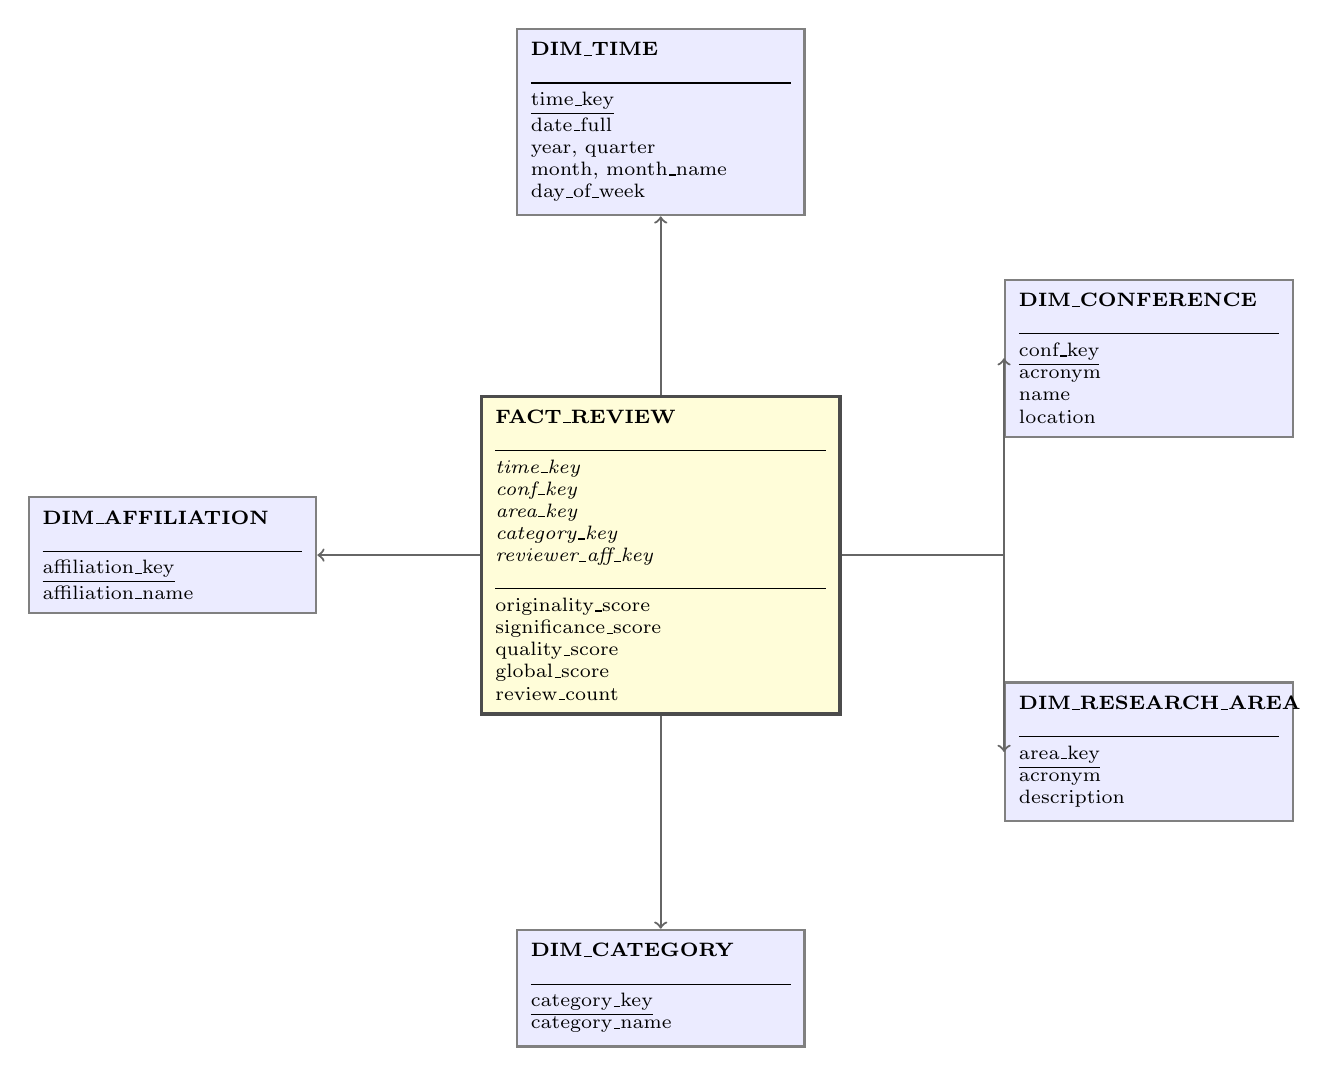
\begin{tikzpicture}[
    fact/.style={
        rectangle, draw=black!70, fill=yellow!15, very thick,
        text width=4.2cm, align=left, font=\scriptsize,
        inner sep=5pt
    },
    dim/.style={
        rectangle, draw=black!50, fill=blue!8, thick,
        text width=3.3cm, align=left, font=\scriptsize,
        inner sep=5pt
    },
    arr/.style={->, thick, black!60}
]

% --- Fact table (center) ---
\node[fact] (fact) at (0,0) {
    \textbf{FACT\_REVIEW} \\[2pt]
    \rule{\linewidth}{0.4pt} \\
    \textit{time\_key} \\
    \textit{conf\_key} \\
    \textit{area\_key} \\
    \textit{category\_key} \\
    \textit{reviewer\_aff\_key} \\[2pt]
    \rule{\linewidth}{0.4pt} \\
    originality\_score \\
    significance\_score \\
    quality\_score \\
    global\_score \\
    review\_count
};

% --- Dimensions ---
\node[dim] (time) at (0, 5.5) {
    \textbf{DIM\_TIME} \\[2pt]
    \rule{\linewidth}{0.4pt} \\
    \underline{time\_key} \\
    date\_full \\
    year, quarter \\
    month, month\_name \\
    day\_of\_week
};

\node[dim] (conf) at (6.2, 2.5) {
    \textbf{DIM\_CONFERENCE} \\[2pt]
    \rule{\linewidth}{0.4pt} \\
    \underline{conf\_key} \\
    acronym \\
    name \\
    location
};

\node[dim] (area) at (6.2, -2.5) {
    \textbf{DIM\_RESEARCH\_AREA} \\[2pt]
    \rule{\linewidth}{0.4pt} \\
    \underline{area\_key} \\
    acronym \\
    description
};

\node[dim] (cat) at (0, -5.5) {
    \textbf{DIM\_CATEGORY} \\[2pt]
    \rule{\linewidth}{0.4pt} \\
    \underline{category\_key} \\
    category\_name
};

\node[dim] (aff) at (-6.2, 0) {
    \textbf{DIM\_AFFILIATION} \\[2pt]
    \rule{\linewidth}{0.4pt} \\
    \underline{affiliation\_key} \\
    affiliation\_name
};

% --- Arrows (Fact -> Dim) ---
\draw[arr] (fact.north)  -- (time.south);
\draw[arr] (fact.east)   -| (conf.west);
\draw[arr] (fact.east)   -| (area.west);
\draw[arr] (fact.south)  -- (cat.north);
\draw[arr] (fact.west)   -- (aff.east);

\end{tikzpicture}
\caption{Star Schema for FACT\_REVIEW.}
\label{fig:star_schema}
\end{figure}

\begin{figure}[!ht]
\centering
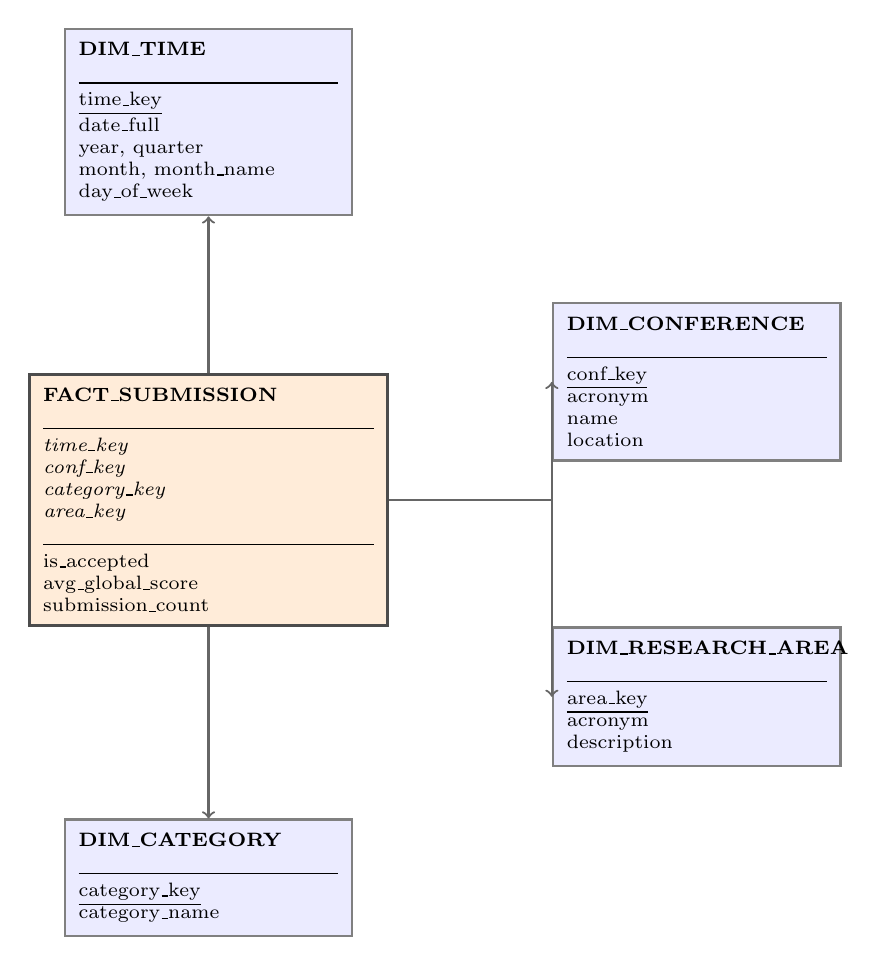
\begin{tikzpicture}[
    fact/.style={
        rectangle, draw=black!70, fill=orange!15, very thick,
        text width=4.2cm, align=left, font=\scriptsize,
        inner sep=5pt
    },
    dim/.style={
        rectangle, draw=black!50, fill=blue!8, thick,
        text width=3.3cm, align=left, font=\scriptsize,
        inner sep=5pt
    },
    arr/.style={->, thick, black!60}
]

% --- Fact table (center) ---
\node[fact] (fact2) at (0,0) {
    \textbf{FACT\_SUBMISSION} \\[2pt]
    \rule{\linewidth}{0.4pt} \\
    \textit{time\_key} \\
    \textit{conf\_key} \\
    \textit{category\_key} \\
    \textit{area\_key} \\[2pt]
    \rule{\linewidth}{0.4pt} \\
    is\_accepted \\
    avg\_global\_score \\
    submission\_count
};

% --- Dimensions ---
\node[dim] (time2) at (0, 4.8) {
    \textbf{DIM\_TIME} \\[2pt]
    \rule{\linewidth}{0.4pt} \\
    \underline{time\_key} \\
    date\_full \\
    year, quarter \\
    month, month\_name \\
    day\_of\_week
};

\node[dim] (conf2) at (6.2, 1.5) {
    \textbf{DIM\_CONFERENCE} \\[2pt]
    \rule{\linewidth}{0.4pt} \\
    \underline{conf\_key} \\
    acronym \\
    name \\
    location
};

\node[dim] (area2) at (6.2, -2.5) {
    \textbf{DIM\_RESEARCH\_AREA} \\[2pt]
    \rule{\linewidth}{0.4pt} \\
    \underline{area\_key} \\
    acronym \\
    description
};

\node[dim] (cat2) at (0, -4.8) {
    \textbf{DIM\_CATEGORY} \\[2pt]
    \rule{\linewidth}{0.4pt} \\
    \underline{category\_key} \\
    category\_name
};

% --- Arrows (Fact -> Dim) ---
\draw[arr] (fact2.north)  -- (time2.south);
\draw[arr] (fact2.east)   -| (conf2.west);
\draw[arr] (fact2.east)   -| (area2.west);
\draw[arr] (fact2.south)  -- (cat2.north);

\end{tikzpicture}
\caption{Star Schema for FACT\_SUBMISSION.}
\label{fig:star_schema_submission}
\end{figure}

\begin{infobox}
FACT\_SUBMISSION does not have a link to DIM\_AFFILIATION because submissions are not tied to a specific reviewer. The two fact tables share the other four dimensions, forming a \emph{constellation schema} (also called galaxy schema).
\end{infobox}

\section{ETL Process}

Data is moved from the operational database to the DW through an ETL (Extract, Transform, Load) process:

\begin{enumerate}
  \item \textbf{Extract}: read new or updated rows from the OLTP tables (Conference, Article, Review, Organizer).
  \item \textbf{Transform}: map natural keys to surrogate keys, compute derived fields like \texttt{is\_accepted}, and extract time components from dates.
  \item \textbf{Load}: insert the transformed rows into the fact and dimension tables.
\end{enumerate}

\begin{infobox}
The ETL runs as a nightly batch job. Real-time updates are not needed because analytical queries are typically run on a daily or weekly basis.
\end{infobox}

\section{OLAP Operations}

With the star schema in place, analysts can perform standard OLAP operations:

\begin{table}[!ht]
\centering
\caption{Standard OLAP operations.}
\label{tab:olap_ops}
\small
\begin{tabularx}{\textwidth}{@{} l X l @{}}
  \toprule
  Operation & What it does & Example \\
  \midrule
  Roll-up    & Go from detail to summary.              & Monthly $\rightarrow$ yearly avg score \\
  Drill-down & Go from summary to detail.              & Conference $\rightarrow$ category level \\
  Slice      & Filter on one dimension.                & Only year 2025 \\
  Dice       & Filter on multiple dimensions.          & Year 2025, location ``Bari'' \\
  Pivot      & Swap rows and columns.                  & Rows = area, Columns = year \\
  \bottomrule
\end{tabularx}
\end{table}
